\documentclass[12pt,a4paper]{article}
\title{A beginners guide to LINUX }
\author{Keno Budde}
\date{\today}
\usepackage{graphicx}
\usepackage{listings}
\usepackage{url}
\usepackage{float}
\begin{document}
\maketitle
\tableofcontents
\section{introduction}
Coming from a non-Unix background I must admit that I had some difficulties getting used to Linux. Nonetheless I can know see the advantages of using a UNIX system. Especially the possibilities of the command line amazed me, in combination with bash scripting. The only thing I think is a shame is that many programs are not available for Linux I really enjoy using daily. Otherwise I would have changed to a Linux distribution as my main operating system. 
\section{the command line}
\begin{figure}[h]
\begin{center}
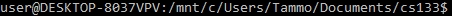
\includegraphics[width=80mm]{./CommandLine.jpg}
\caption{now my favorite tool}
\label{CommandLine}
\end{center}
\end{figure}
The command line is the UNIX tool I felt the most uncomfortable with on my first day of using a linux distribution but it became the tool I enjoy now the most. What techrepublic can say about command line applications was exactly how I experienced my life with this tool: ``Beginners can learn the rudimentary basics easily, and as they learn more about how to use it their facility with the application expands. '' \cite{CommandLineTools11} I began to enjoy the possibilities I would have using the terminal and the time I would gain in comparison to working on my windows operating system. I take pleasure in easily moving around files and directories with simple commands without having to drag and drop them around. The five commands I got the most comfortable with in the short amount of time I should call the first term are the following:
\begin{enumerate}
\item \textbf{ssh}: using ssh or the secure shell is something I got very used to especially when working. ssh allows a user to securely log into a remote system. Using the \textbf{-Y} option to enable X11 forwarding it is even possible to see a graphical remote desktop. An example for that command would be the way I could log onto the server of the department of computer science, Joshua. 
\begin{center}
\begin{tabular}{c}
\begin{lstlisting}[language=bash]
  $ ssh -Y u1632823@joshua.dcs.warwick.ac.uk
\end{lstlisting}
\end{tabular}
\end{center}
\item \textbf{git}: another very important program for me I want to talk about later in this guide is git. Using it as a version control tool saved my work multiple times when I could roll back to the last working version.
\item \textbf{man}: while trying to get to know Linux my best helper were manual pages of the commands I wanted to use. I first had to get used to the way they are written but now they are an essential asset for my work. Working on a bash program the other day I wanted to get to know the sort command, so the first thing I did was to consult the manual page of the command. 
\begin{figure}[h]
\begin{center}
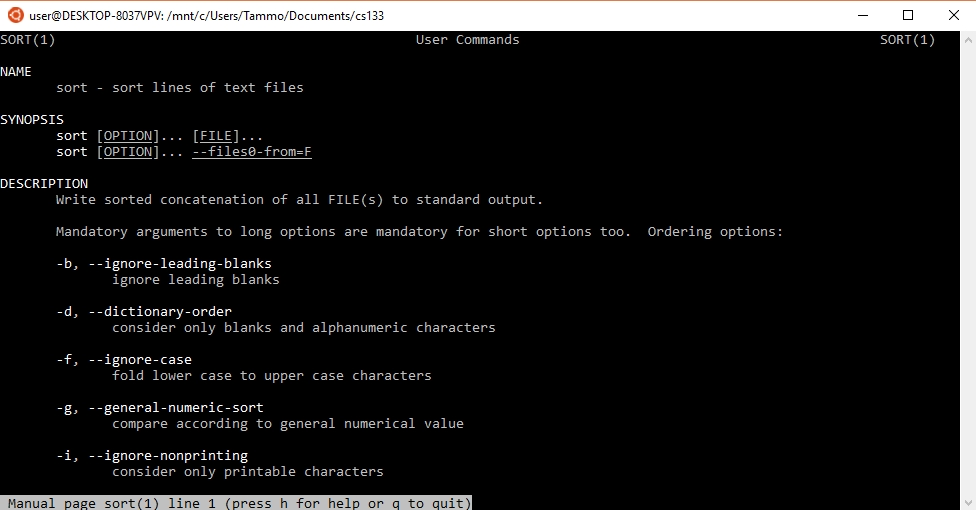
\includegraphics[width=150mm]{./manual.jpg}
\label{SortManual}
\end{center}
\end{figure} 
\item \textbf{lpr}: printing out my work for various assignments I really enjoyed the ease of use of the lpr command which enables the user to print a file easily. To actually print a document it is only necessary to specify the printer and the document I wish to print: 
\begin{center}
\begin{tabular}{c}
\begin{lstlisting}[language=bash]
  $ lpr -Pdcs001a info.pdf
\end{lstlisting}
\end{tabular}
\end{center}
\item \textbf{cd}: an essential command to navigate is cd and its ease of use is wonderful. To navigate somewhere, it is possible to give the command an absolute path, which could be something like this:
\begin{center}
\begin{tabular}{c}
\begin{lstlisting}[language=bash]
  $ cd /mnt/c/Users/Public
\end{lstlisting}
\end{tabular}
\end{center}
Another possibility to use this command is to give it a relative path to work with, an example is shown below:

\begin{center}
\begin{tabular}{c}
\begin{lstlisting}[language=bash]
  $ cd ../Documents/cs132
\end{lstlisting}
\end{tabular}
\end{center}
\end{enumerate}
\section{version control}
As I mentioned above over the last months I took a lot of pleasure from working with git as a version control software. It saved my work more than once and it was also very motivating for me to see the statistics of my progress online through my github.com calendar. After reading up a bit more about git and its possibilities as a tool for programmers I created an account on github to use it as a backup for the files I am working on. Working with git is really easy. The repository to work on has first to be intialized for git:

\begin{center}
\begin{tabular}{c}
\begin{lstlisting}[language=bash]
  $ git init sample_directory
\end{lstlisting}
\end{tabular}
\end{center}
If if been working on this project before without starting git from the beginning I would have to add all files to git, otherwise I could specify specific files:
\begin{center}
\begin{tabular}{c}
\begin{lstlisting}[language=bash]
  $ git add *
\end{lstlisting}
\end{tabular}
\end{center}
After that the first commit has to be made:
\begin{center}
\begin{tabular}{c}
\begin{lstlisting}[language=bash]
  $ git commit -m "created directory and documentation files"
\end{lstlisting}
\end{tabular}
\end{center}
More often than not I am using a service like github.com to backup my work. This means
that the remote service has to be set up: 
\begin{center}
\begin{tabular}{c}
\begin{lstlisting}[language=bash]
$ git remote add origin url
# sets a new remote server
$ git remote -v
# verifies the new service  
\end{lstlisting}
\end{tabular}
\end{center}
Another useful feature I learned about is the possibility to take a look at a previous commit. \cite{OldCommits} Therefore
the git log feature makes it easy to have a better look at the commits:
\begin{center}
\begin{tabular}{c}
\begin{lstlisting}[language=bash]
  $ git log --oneline
\end{lstlisting}
\end{tabular}
\end{center}
By ``checking out'' to a previous commit it is possible to have a look at the way the code looked the time the commit was done.
\begin{center}
\begin{tabular}{c}
\begin{lstlisting}[language=bash]
  $ git checkout commit
\end{lstlisting}
\end{tabular}
\end{center}
If I want to do an experiment I usually create a new branch to experiment on.
\begin{center}
\begin{tabular}{c}
\begin{lstlisting}[language=bash]
$ git branch experiment
# creates a new branch called experiment
$ git checkout experiment
# checks out the experiment branch which means that
# the user is working now on this branch  
\end{lstlisting}
\end{tabular}
\end{center}
When I am happy with the experiments I made and tested them I can now reinclude those changes into the master branch. Therefore
I can rebase now the experiment branch into the master branch and merge them together \cite{GitBranch}:
\begin{center}
\begin{tabular}{c}
\begin{lstlisting}[language=bash]
$ git rebase master
# rebases the experiment branch to the master branch
$ git checkout master
# checks out the master branch
$ git merge experiment
# merges the two branches together  
\end{lstlisting}
\end{tabular}
\end{center}
\begin{figure}[H]
\begin{center}
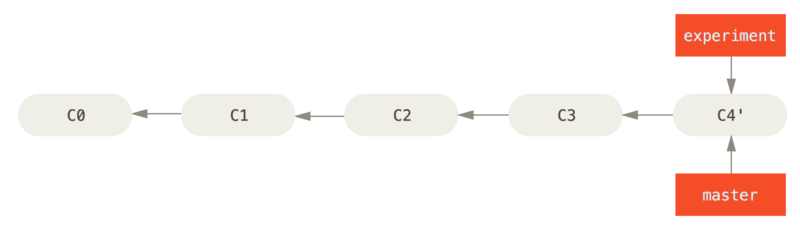
\includegraphics[width=\textwidth]{./basic-rebase-4.png}
\caption{Forwarding the master branch \cite{GitBranch}}
\label{BasicRebase}
\end{center}
\end{figure}
\section{useful commands and programs}
Following up on the short list of the commands I mentioned in a previos section I want to talk about a few more useful commands and programs I enjoy using.
\begin{itemize}
\item \textbf{cp}: Enables the user to copy files. 
\begin{center}
\begin{tabular}{c}
\begin{lstlisting}[language=bash]
$ cp index.html index2.html
# copies index.html into a second file 
# called index2.html
\end{lstlisting}
\end{tabular}
\end{center}
\item \textbf{mv}: Enables the user to move and rename files. 
\begin{center}
\begin{tabular}{c}
\begin{lstlisting}[language=bash]
$ mv index.html index2.html
# renames index.html into index2.html
\end{lstlisting}
\end{tabular}
\end{center}
\item \textbf{export}: Enables the user to set an environmental variable. For example this command could be used to set include a new manual page:

\begin{center}
\begin{tabular}{c}
\begin{lstlisting}[language=bash]
$ export MANPATH=$(man -w):~/lab1resources/man
\end{lstlisting}
\end{tabular}
\end{center}
\item \textbf{mkdir}: creates a new directory. For example when I created the public\_html directory I used this command:

\begin{center}
\begin{tabular}{c}
\begin{lstlisting}[language=bash]
$ mkdir public_html
\end{lstlisting}
\end{tabular}
\end{center}
\item \textbf{chmod}: changes permissions of files or directories. Can be used with an octal number or the explicit access permissions:

\begin{center}
\begin{tabular}{c}
\begin{lstlisting}[language=bash]
$ chmod 644 index.html
# changes the permissions to read/write 
# for the owner, read only for users 
# in the group and others
\end{lstlisting}
\end{tabular}
\end{center}
\item \textbf{ls}: lists files in the current directory. The command can be modified to list hidden file or to work recursively:

\begin{center}
\begin{tabular}{c}
\begin{lstlisting}[language=bash]
$ ls -all
# lists all files in the directory including
# hidden files
\end{lstlisting}
\end{tabular}
\end{center}
\item \textbf{touch}: creates a plain text file.
\item \textbf{expr}: can be used to evaluate arithmetic expressions. For expample the following equation can be solved by this command:
\begin{equation}
5 + 5 = x
\end{equation}
Using the command \textbf{expr} this like any other basic arithmetic expressions.
 
\begin{center}
\begin{tabular}{c}
\begin{lstlisting}[language=bash]
$ expr 5 + 5
$ 10
\end{lstlisting}
\end{tabular}
\end{center}
\end{itemize}
\bibliographystyle{plain}
\bibliography{references}
\end{document}

